\documentclass[a4, 12pt, UTF8]{ctexart}

\usepackage[english]{babel}
\usepackage{setspace}
\usepackage{hyperref}
\usepackage[margin=1.5in]{geometry}
\usepackage{amsmath}
\usepackage{amsthm}
\usepackage{amsfonts}
\usepackage{amssymb}
\usepackage[usenames,dvipsnames]{xcolor}
\usepackage{graphicx}
\usepackage{hyperref}
\usepackage[numbers, square]{natbib}
\usepackage{fancybox}
\usepackage{picins}
\usepackage{picinpar}
\usepackage{epsfig}
\usepackage{epstopdf}
\graphicspath{{figure/section1/}{figure/section2/}{figure/section3/}}
\usepackage{fancyhdr}
\newcommand{\red}{\textcolor{red}}
\newcommand{\blue}{\textcolor{blue}}

\setlength{\baselineskip}{20pt}

\pagestyle{fancy}



\title{贡嘎环线徒步计划}

\begin{document}
  \maketitle

  \renewcommand{\contentsname}{目录}
  \renewcommand{\refname}{参考文献}

  \tableofcontents

  \section{前期准备}
\subsection{贡嘎环线}

\begin{figure}[htbp]
  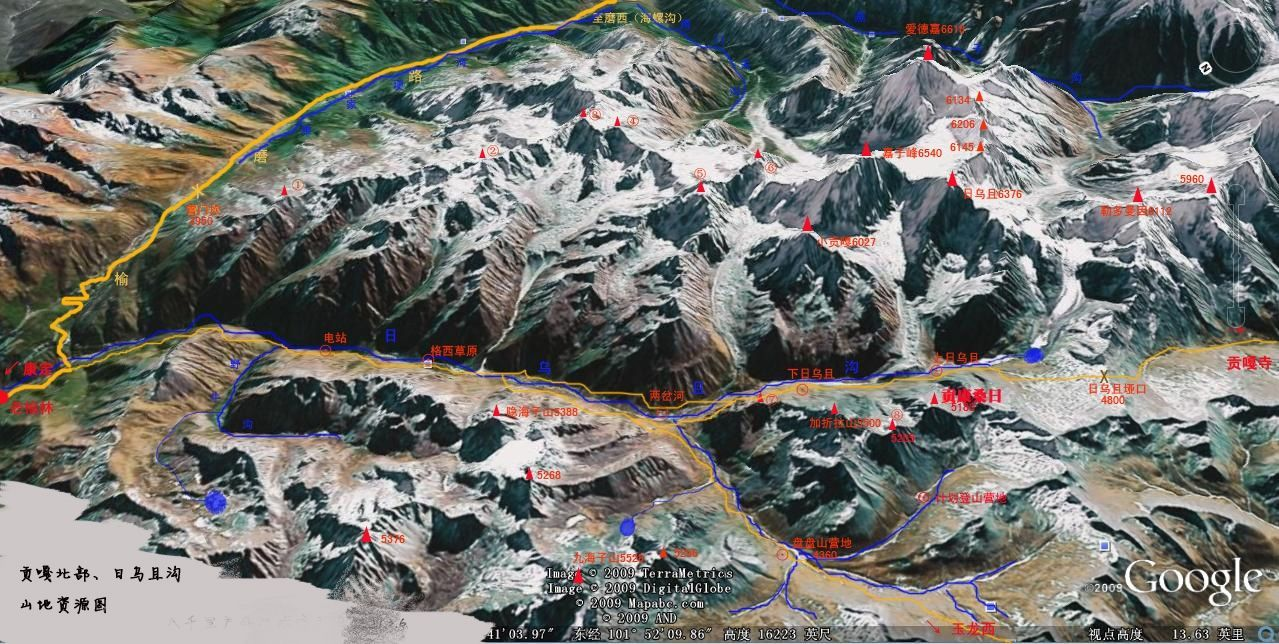
\includegraphics[width=1.0\textwidth]{shandi.jpg}
\end{figure}
\begin{figure}[htbp]
  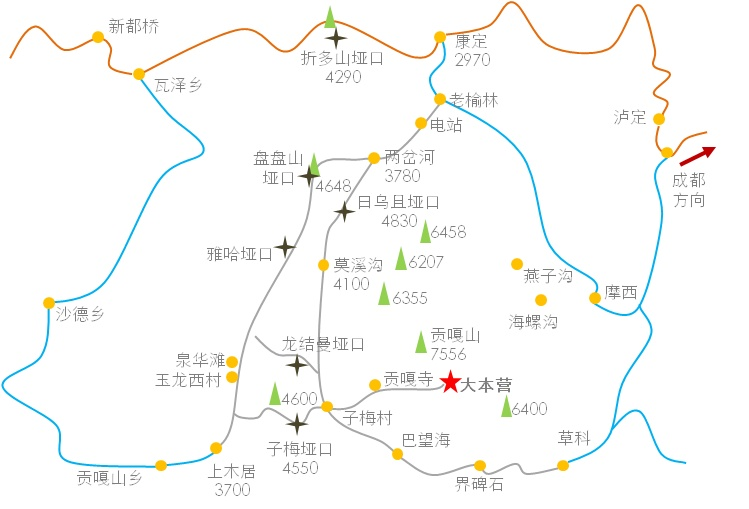
\includegraphics[width=1.0\textwidth]{map1.jpg}
\end{figure}
\begin{figure}[htbp]
  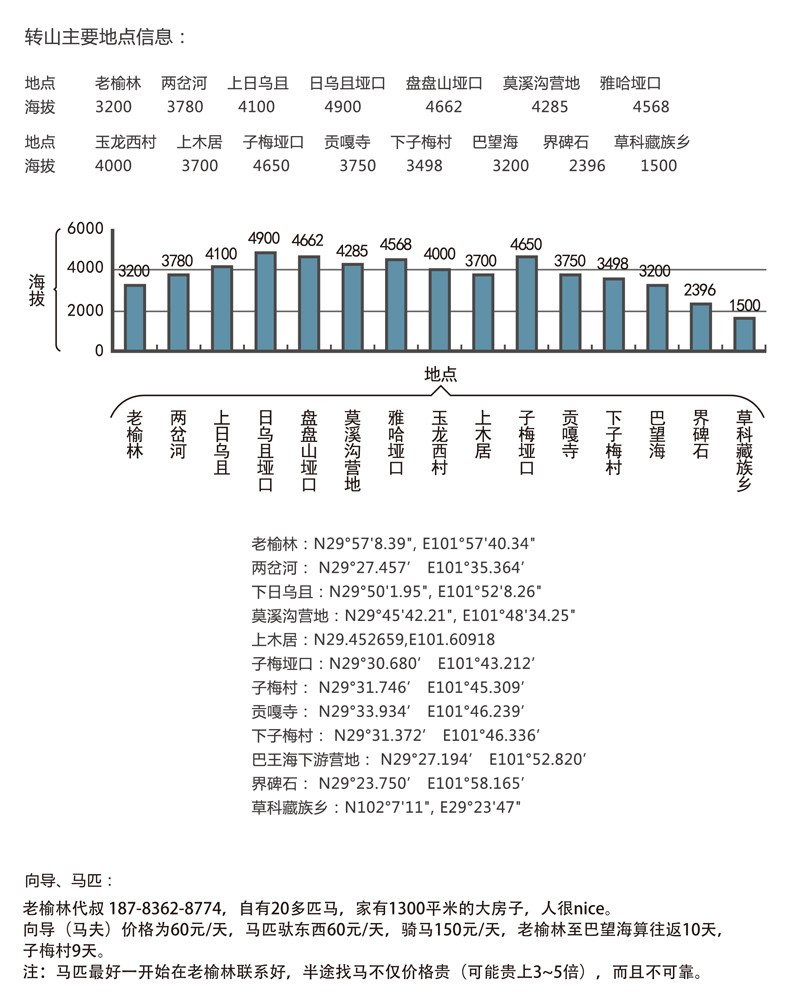
\includegraphics[width=1.0\textwidth]{inf.jpg}
\end{figure}

\subsection{装备购置}
\subsubsection{服装装备}
\begin{itemize}
  \item 冲锋衣(防风,防水,透气,耐磨)
  \item 抓绒衣 (含windstopper,防风保暖)
  \item 排汗内衣(保持身体干燥,防止失温)
  \item 羽绒衣裤,雨衣
  \item 个人衣物(一次性内裤,等)
  \item 徒步鞋, 溯溪鞋,登山鞋
  \item 排汗袜 (最好是coolmax面料,配合gore-tex穿,可排脚汗,防冻伤和起水泡)
  \item 遮阳帽,抓绒帽,厚手套,雪镜或墨镜,头巾
\end{itemize}
\subsubsection{辅助装备}
\begin{itemize}
  \item 保温水壶
  \item 头灯,手电
  \item 登山杖
  \item 护膝
  \item 雪套?(在雪地和泥泞的公路很管用?)
  \item 登山包(建议60升或以上),冲锋包?(小包,背负路餐及其他用品),可能要驮包?(用以马托运)
  \item 防水袋
  \item 纸质地图,指南针,军刀,求生哨,对讲机
  \item 打火机
\end{itemize}
\subsubsection{露营装备}
\begin{itemize}
  \item 睡袋(极限温标至少-15度以下)
  \item 帐篷(四季帐或高山帐),帐灯?
  \item 帐篷地席(保护你的帐篷底面,免受磨损)
  \item 防潮垫(泡沫垫或充气垫)
  \item 铝膜地席(选择性带)
  \item 炉头,气罐,套锅(用于烧水煮茶),高压锅?
\end{itemize}
\subsubsection{医疗用品}
\begin{itemize}
  \item 处方药:乙酰唑胺、综合维他命、硝苯地平和低塞米松--处方药,有副作用,需在药师指导下依照个人情况服用\\
        乙酰唑胺可增加肺通气量,提高血氧饱和度和睡眠质量。乙酰唑胺可减轻高原病症状,有降低高原病发病率的倾向。地塞米松属于短期防治急性高原反应的药物。地塞米松能预防急性高原病,可以预防高原肺水肿的发生。\\
        非处方药:阿司匹林、芬必得--镇痛药,对缓解高反引起的头痛有较好的疗效,可以相应地改善身处高海拔营地时的睡眠质量;红景天可以增加血液流动性,改善缺氧,改善高反状况。\\
        救生毯--可以隔绝皮肤与寒冷空气的接触,其含有的金属成分可以反射身体的热辐射,最大限度锁住身体热量的流失,避免失温加剧。
\end{itemize}
\subsubsection{生活用品}
\begin{itemize}
  \item 餐具
  \item 路餐
  \item 贴身
\end{itemize}
\subsubsection{其他}
\begin{itemize}
  \item 移动电源,数据线
  \item 学生证,身份证
  \item 真空袋,环保袋,卫生纸
  \item 打火石,镊子
  \item 军刀
\end{itemize}

\subsection{相关网址}
\begin{itemize}
  \item 如何制作手机离线地图?\\
   \url{http://www.8264.com/wenzhang/5510614.html}
  \item 徒步也有套路:7种不同路面,7种徒步技巧\\
    \url{http://www.8264.com/viewnews-128290-page-1.html}
\end{itemize}
\subsection{训练计划}

  \section{徒步行程}
\subsection{路线安排}
路线1
\begin{itemize}
  \item Day 1: 成都-147km-雅安-168km-泸定-49km-康定-75km-新都桥(也可以选择住康定)
  \item Day 2: 新都桥-20km-甲跟坝-43km-沙德-99km-六巴-上木居-10km-泉华滩-6km-冷嘎措-玉龙西村(或者上木居)
  \item Day 3: 玉龙西村-玉龙西村徒步入口-龙洁曼垭口-莫西沟-贡嘎寺
  \item Day 4: 贡嘎寺-7km-子梅村-11km-巴望海-7km-公路出口-25km-草科乡(-58km-石棉)
  \item Day 5: 草科乡-58km-石棉-196km雅安-60km-(平安古镇)-95km-成都
\end{itemize}
路线2
\begin{itemize}
  \item Day 1: 成都-雅安-康定-新都桥
  \item Day 2: 新都桥-格西草原(3400m)-下日乌且草原(h4200m)
  \item Day 3: 下日乌且营地-上日乌且-日乌且垭口(h4925m)-莫溪沟冬季牧场(h3800-3900m)
  \item Day 4: 冬季牧场营地-西柑牧场-贡嘎寺(h3500m)
  \item Day 5: 贡嘎寺-子梅村-子梅垭口-巴望海-草科乡
  \item Day 6: 草科乡-成都
\end{itemize}
路线3
\begin{itemize}
  \item Day 1: 成都-137km-雅安-213km-康定-10km-老榆林-8km-电站-3km-格西草原
  \item Day 2: 格西草原-8km-两汾河(h3780m)-5km-下日乌且-4km-上日乌且
  \item Day 3: 上日乌且-4km-日乌且垭口-6km-莫溪沟尾营地
  \item Day 4: 莫溪沟尾营地-12km-西柑牧场
  \item Day 5: 西柑牧场-7km-贡嘎寺-5km-下子梅村(客栈)
  \item Day 6: 下子梅村-7km-巴望海-4km-界碑石-18km-草科-石棉
  \item Day 7: 石棉-267km-成都
\end{itemize}
路线4
\begin{itemize}
  \item Day 1: 成都-雅安-二郎山-泸定-康定-老榆林-电站-3km-格西草原
  \item Day 2: 格西草原-8km-两汾河-5km-下日乌且-4km-上日乌且
  \item Day 3: 上日乌且-6km-日乌且垭口-12km-莫溪沟尾营地
  \item Day 4: 莫溪沟尾营地-14km-冬季牧场尾-11km-贡嘎寺
  \item Day 5: 贡嘎寺-8km-下子海村-11km(乘车)-子海垭口-11km(乘车)-下子海村
  \item Day 6: 下子海村-11km-巴旺海-7km-界碑石-草科或石棉
  \item Day 7: 草科或石棉-雅安-成都
\end{itemize}
备选路线(如因大雪导致日乌且垭口无法通过):
\begin{itemize}
  \item Day 1: 成都-康定-格西草原
  \item Day 2: 格西草原-两汾河-盘盘山营地
  \item Day 3: 盘盘山营地-垭口-玉龙西村
  \item Day 4: 玉龙西村-泉华滩-子梅垭口-子梅村
  \item Day 5: 子梅村-贡嘎寺-下子海村
  \item Day 6: 下子海村-巴望海-草科-石棉
  \item Day 7: 石棉-成都
\end{itemize}


  \section{意外应对}


\bibliographystyle{nature}
\bibliography{ref}
\end{document} 